\chapter{Macrovectors}
\label{appendix:macrovectors}

\begin{figure}
  \centering
  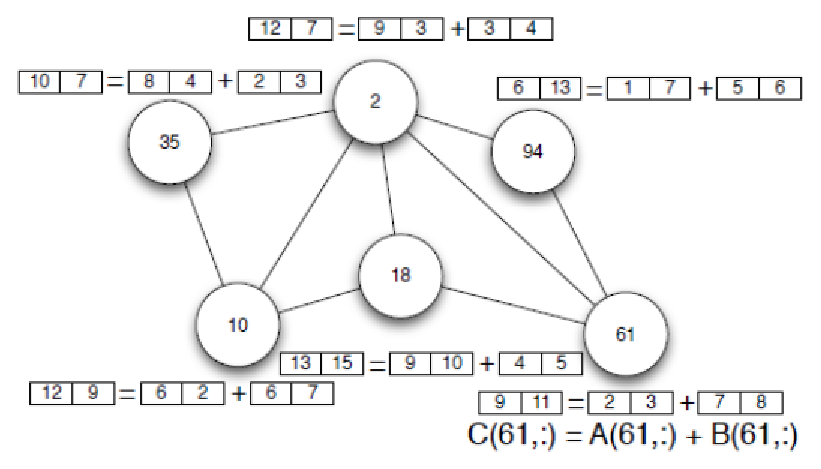
\includegraphics[width=0.8\columnwidth]{fig/DistributedArray.eps}
  \caption[Distributed Macrovector]{Distributed Macrovector: Nodes can read and write their own values in
  the vector.}
  \label{fig:distributedVector}
\end{figure}

\begin{figure}
  \centering
  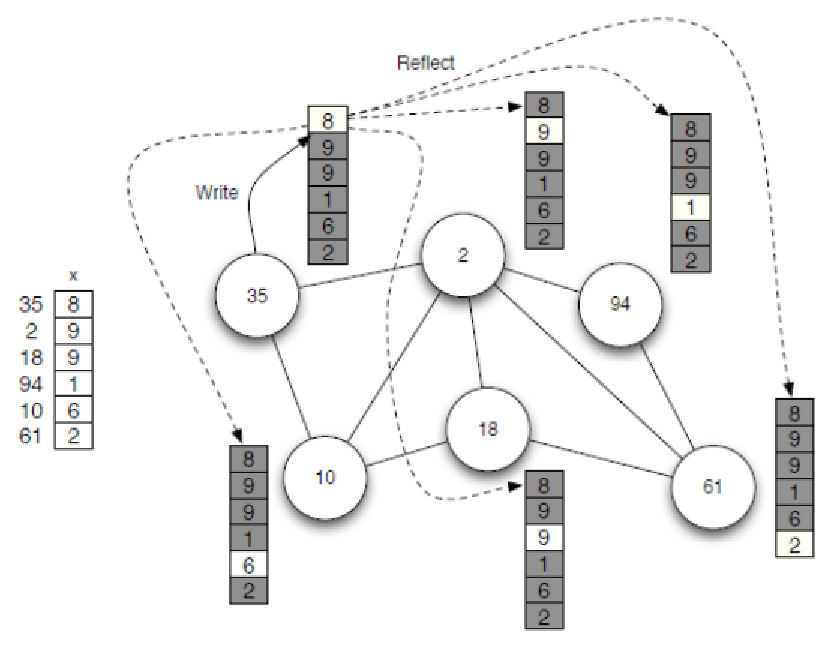
\includegraphics[width=0.8\columnwidth]{fig/ReflectedArray.eps}
  \caption[Reflected Macrovector]{Reflected Macrovector: Nodes can read all values in the vector, but can only write to their own value.}
  \label{fig:reflectedVector}
\end{figure}

% \begin{figure}
%   \centering
%   \subfigure[Distributed Macrovector: Nodes can read and write their own
%   values in the vector.]{
%   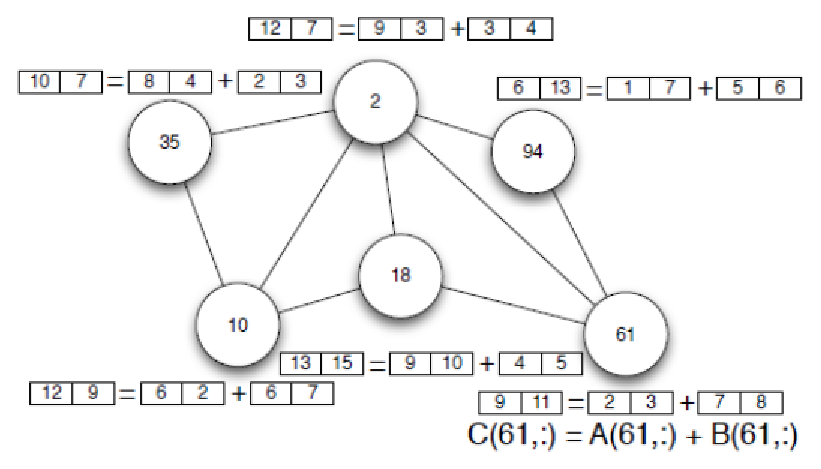
\includegraphics[width=0.8\columnwidth]{fig/DistributedArray.eps}
%   \label{fig:distributedVector}
%   } \subfigure[Reflected Macrovector: Nodes can read all values in the vector,
%   but can only write to their own value.]{
%   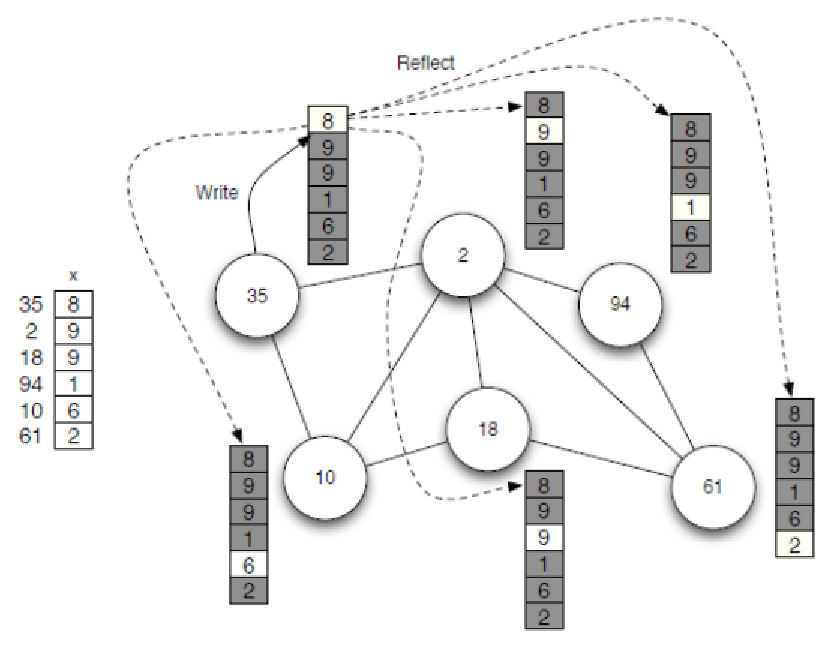
\includegraphics[width=0.8\columnwidth]{fig/ReflectedArray}
%   \label{fig:reflectedVector}
%   }
%   \caption[Example macrovector representations]{Macrovectors can be
%     (a) distributed across nodes or (b) reflected across nodes. They
%     can also be represented in other ways that are not shown.}
% \end{figure}
